
\documentclass[a4paper,11]{article}

%\title{Unused Title}
\usepackage{graphicx}
\usepackage{hyperref}
\usepackage{multirow}
\usepackage{multicol}
\usepackage{blindtext}
\usepackage[utf8]{inputenc}
\usepackage[english]{babel}
\usepackage[T1]{fontenc}

% Use helvet if uarial cannot be installed
%\usepackage{uarial}
\usepackage[scaled]{helvet}

\renewcommand{\familydefault}{\sfdefault}
\usepackage{amssymb}
\usepackage{amsmath}
\usepackage{courier}
\usepackage{setspace}
\usepackage[table,svgnames]{xcolor}
\usepackage{fancyvrb} 
\usepackage{listings}
\usepackage{caption}
\usepackage{longtable}
\usepackage{relsize}
\usepackage{tfrupee}
\usepackage{rotating}
\usepackage{lipsum}
\usepackage{subcaption}
\usepackage{float}
\usepackage{aliascnt}


\usepackage{natbib}
\newcommand*{\urlprefix}{Available from: }
\newcommand*{\urldateprefix}{Accessed }
\bibliographystyle{bath}
\renewcommand{\bibsection}{}

\makeatletter
\newcommand\footnoteref[1]{\protected@xdef\@thefnmark{\ref{#1}}\@footnotemark}
\makeatother

\newaliascnt{eqfloat}{equation}
\newfloat{eqfloat}{h}{eqflts}
\floatname{eqfloat}{Equation}

\newcommand*{\ORGeqfloat}{}
\let\ORGeqfloat\eqfloat
\def\eqfloat{%
	\let\ORIGINALcaption\caption
	\def\caption{%
		\addtocounter{equation}{-1}%
		\ORIGINALcaption
	}%
	\ORGeqfloat
}

\addto\captionsenglish{% Replace "english" with the language you use
	\renewcommand{\contentsname}%
	{List of Contents}%
}

\newcommand\tab[1][1cm]{\hspace*{#1}}

\definecolor{codegreen}{rgb}{0,0.6,0}
\definecolor{codegray}{rgb}{0.5,0.5,0.5}
\definecolor{codepurple}{rgb}{0.58,0,0.82}
\definecolor{backcolour}{rgb}{0.95,0.95,0.92}

\lstdefinestyle{mystyle}{
	backgroundcolor=\color{backcolour},   
	commentstyle=\color{codegreen},
	keywordstyle=\color{magenta},
	numberstyle=\tiny\color{codegray},
	stringstyle=\color{codepurple},
	basicstyle=\ttfamily\footnotesize,
	breakatwhitespace=false,         
	breaklines=true,                 
	captionpos=b,                    
	keepspaces=true,                 
	numbers=left,                    
	numbersep=5pt,                  
	showspaces=false,                
	showstringspaces=false,
	showtabs=false,                  
	tabsize=2,
	xleftmargin=0.5cm,
	xrightmargin=-0.8cm,
	frame=lr,
	%	framesep=-5pt,
	framerule=0pt
}

\lstset{style=mystyle}

\definecolor{Teal}{RGB}{0,128,128}
\definecolor{NewBlue1}{RGB}{4,100,226}
\definecolor{NiceBlue}{RGB}{63,104,132}
\definecolor{DarkRed}{RGB}{14,53,59}
\definecolor{NewBlue2}{RGB}{62,100,125}
\definecolor{NewBlue3}{RGB}{44,100,128}

\hypersetup{
	colorlinks,
	citecolor=NiceBlue,
	linkcolor=NewBlue1,
	urlcolor=Blue
	%	citebordercolor=Violet,
	%	filebordercolor=Red,
	%	linkbordercolor=Blue
}

\usepackage{geometry}
\linespread{1.25}
\usepackage[parfill]{parskip} % Avoid indentation

\geometry{
	a4paper,
	left=4cm,
	right=2.5cm,
	top=2.5cm,
	bottom=2.5cm,
}


\begin{document}
	\pagenumbering{gobble}
	\begin{center}
		{\large IMPERIAL COLLEGE BUSINESS SCHOOL}
	\end{center}
	%	\maketitle
	\vspace{6cm}
	
	\begin{center}
		
		\Huge This is the title to the paper which can span multiple lines\\		
		\vspace{.5cm}		
		\large {Word Count: 1,000}
		
	\end{center}
	\vspace{2.5cm}
	\begin{center}
		\Large John Doe\\Advisor: Dr. James Doe
	\end{center}
	
	\vspace{8cm}
	\begin{center}
		{\large A report submitted in partial fulfilment of the \\requirements for the MSc Business Analytics degree}
	\end{center}
	
	\begin{center}
		{\large August 2020}
	\end{center}		

	\newpage
	\pagenumbering{Roman}

\section{How to use this template (Comment section before use)}

\textbf{Imperial College London Business School: Template for : Individual Research Report, MS, Business Analytics, 
}

\textbf{Template Disclaimer}

By making use of any template, you agree to the following:

NO WARRANTIES: All of the information provided on this template is provided "AS-IS" and with NO WARRANTIES. No express or implied warranties of any type, including for example implied warranties of merchantability or fitness for a particular purpose, are made with respect to the information, or any use of the information, on this template. Parties involved in preparing the template makes no representations and extends no warranties of any type as to the accuracy or completeness of any information or content on this template.


DISCLAIMER OF LIABILITY: All parties involved in preparing the document specifically DISCLAIMS LIABILITY FOR INCIDENTAL OR CONSEQUENTIAL DAMAGES OF ANY KIND and assumes no responsibility or liability for any loss or damage suffered as a result of the use or misuse of any of the information or content in this template. The parties involved in preparing the document assumes or undertakes NO LIABILITY for any loss or damage suffered as a result of the use, misuse or reliance on the information and content on this template. Use at your own risk.

{\color{red} \rule{\linewidth}{0.5mm} }
\textcolor{red}{\textbf{COMMENT THE FOLLOWING LINES IN THE TEMPLATE TO HIDE HOW-TO SECTION}}
\begin{verbatim}
\section{How to use this template (Comment section before use)}

\textbf{Imperial College London Business School: Template for : Individual Research Report, MS, Business Analytics, 
}

\textbf{Template Disclaimer}

By making use of any template, you agree to the following:

NO WARRANTIES: All of the information provided on this template is provided "AS-IS" and with NO WARRANTIES. No express or implied warranties of any type, including for example implied warranties of merchantability or fitness for a particular purpose, are made with respect to the information, or any use of the information, on this template. Parties involved in preparing the template makes no representations and extends no warranties of any type as to the accuracy or completeness of any information or content on this template.


DISCLAIMER OF LIABILITY: All parties involved in preparing the document specifically DISCLAIMS LIABILITY FOR INCIDENTAL OR CONSEQUENTIAL DAMAGES OF ANY KIND and assumes no responsibility or liability for any loss or damage suffered as a result of the use or misuse of any of the information or content in this template. The parties involved in preparing the document assumes or undertakes NO LIABILITY for any loss or damage suffered as a result of the use, misuse or reliance on the information and content on this template. Use at your own risk.

{\color{red} \rule{\linewidth}{0.5mm} }
\textcolor{red}{\textbf{COMMENT THE FOLLOWING LINES IN THE TEMPLATE TO HIDE HOW-TO SECTION}}
\begin{verbatim}
\section{How to use this template (Comment section before use)}

\textbf{Imperial College London Business School: Template for : Individual Research Report, MS, Business Analytics, 
}

\textbf{Template Disclaimer}

By making use of any template, you agree to the following:

NO WARRANTIES: All of the information provided on this template is provided "AS-IS" and with NO WARRANTIES. No express or implied warranties of any type, including for example implied warranties of merchantability or fitness for a particular purpose, are made with respect to the information, or any use of the information, on this template. Parties involved in preparing the template makes no representations and extends no warranties of any type as to the accuracy or completeness of any information or content on this template.


DISCLAIMER OF LIABILITY: All parties involved in preparing the document specifically DISCLAIMS LIABILITY FOR INCIDENTAL OR CONSEQUENTIAL DAMAGES OF ANY KIND and assumes no responsibility or liability for any loss or damage suffered as a result of the use or misuse of any of the information or content in this template. The parties involved in preparing the document assumes or undertakes NO LIABILITY for any loss or damage suffered as a result of the use, misuse or reliance on the information and content on this template. Use at your own risk.

{\color{red} \rule{\linewidth}{0.5mm} }
\textcolor{red}{\textbf{COMMENT THE FOLLOWING LINES IN THE TEMPLATE TO HIDE HOW-TO SECTION}}
\begin{verbatim}
\section{How to use this template (Comment section before use)}
\input{howtouse.tex}
\pagebreak
\end{verbatim}
{\color{red} \rule{\linewidth}{0.5mm}}

\textcolor{red}{\textbf{FONT USAGE}}

The Arial font is recommended for the Individual Research Report. However, this needs to be installed manually as discussed in this document. For Overleaf, Helvetica has been used. If you are able to install Arial, comment the line \texttt{usepackage[scaled]\{helvet\}} and uncomment \texttt{usepackage\{uarial\}}.

{\color{red} \rule{\linewidth}{0.5mm}}

\textbf{FORMATTING AND PAGE NUMBERING CONVENTIONS USED}

\begin{itemize}
	\item Geometry
	\begin{itemize}
		\item left-hand margin of 4 cm;
		\item right-hand margin of 2.5cm (1 inch);
		\item top margin 2.5cm (1 inch);
		\item bottom margin 2.5cm (1 inch).
	\end{itemize}
	\begin{itemize}
		\item The Synopsis, Acknowledgements, List of Contents and Notation should be numbered with upper case Roman Numerals.
		\item The main text, starting with the first page of the first chapter (or Introduction) should be numbered, starting with page 1, using Arabic Numerals, through to the end of the references.
		\item \textbf{Appendices should be numbered using lower case Roman Numerals. -- Check to make sure this is what is needed. If not comment \texttt{\\pagenumbering\{roman\}} in template before Appendix}
	\end{itemize}
	\item Pages must be numbered at the bottom centre of the page.
	\item The title page should be blank.
\end{itemize}

\subsection{Prerequisites}

There are 2 primary pre-requisites: First, to install the Bath BibTeX style and second to install the Arial font. Note that if Arial cannot be installed, it may be possible to use Helvetica if the department agrees 

\textbf{1. Install the Bath BibTeX style (See Included Folder)}

\textbf{2. Install Font Arial}: See \hyperlink{https://www.tug.org/fonts/getnonfreefonts/}{https://www.tug.org/fonts/getnonfreefonts/} and 

\textbf{Notes from \hyperlink{https://tex.stackexchange.com/questions/37120/how-can-i-install-uarial-sty-on-a-mac}{Install uarial on a Mac} question on Stackexchange: }

The font can be easily installed via the script getnonfreefonts. It is available at tug.org: \hyperlink{http://www.tug.org/fonts/getnonfreefonts/}{getnonfreefonts}. I tried the installation of \hyperlink{http://www.tug.org/fonts/getnonfreefonts/install-getnonfreefonts}{getnonfreefonts} on my Mac.

\begin{itemize}
	\item Install MacTeX 
	\item Download the installation script. Open the terminal and go to the folder Download
	
	\texttt{cd Download}
	\item Run the installation: \texttt{sudo texlua install-getnonfreefonts}
	
	The installation finished and the scipts with their execute files getnonefreefonts and getnonfreefonts-sys are now located at \texttt{/usr/local/texlive/2011/bin/x86\_64-darwin/}
	
	\item Now you can run the script \texttt{sudo getnonfreefonts-sys -a}
\end{itemize}

\subsection{Images}
\begin{figure*}[!ht]
	\centering
	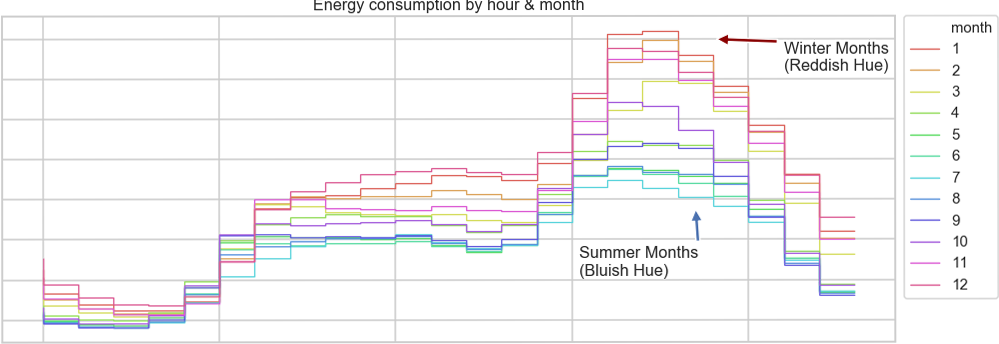
\includegraphics[width=16cm]{images/testimage1}
	\caption{This is an image}
	\label{fig:testimage1}
\end{figure*}

\begin{figure*}[!ht]
	\centering
	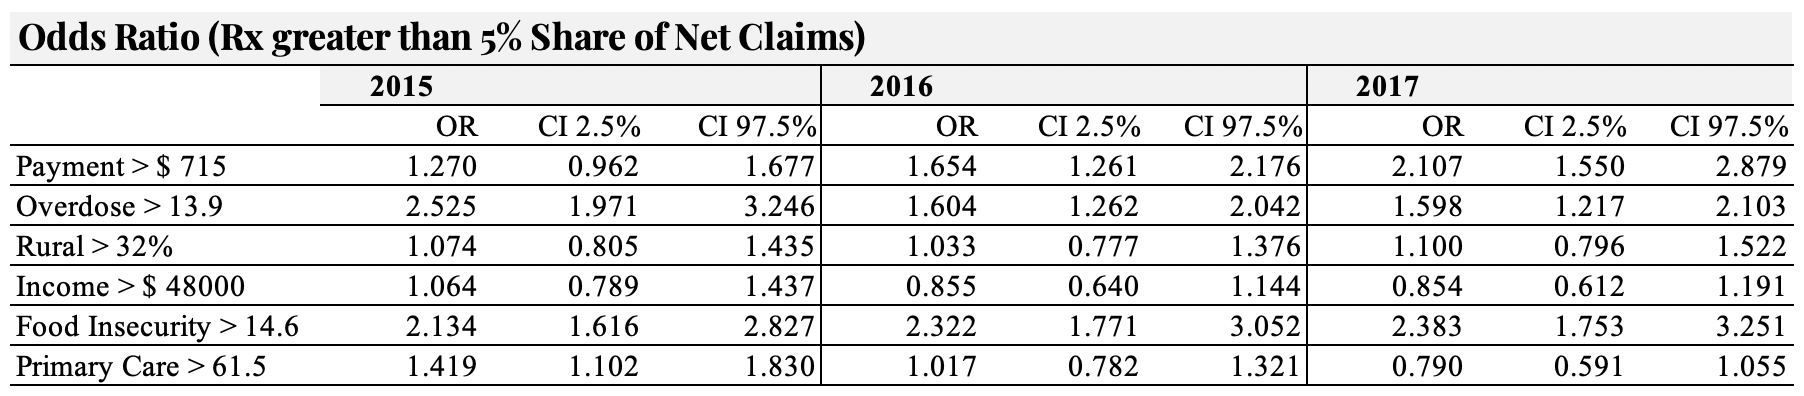
\includegraphics[width=16cm]{images/testimage2}
	%	\caption{Round 1 Blue Strategy to increase Market Share}
	\captionof{table}[This is a table shown as an image]{This is a table shown as an image}
	\label{fig:testimage2}
\end{figure*}

\begin{figure*}[!ht]
	\centering
	\subfloat[A floating image]{{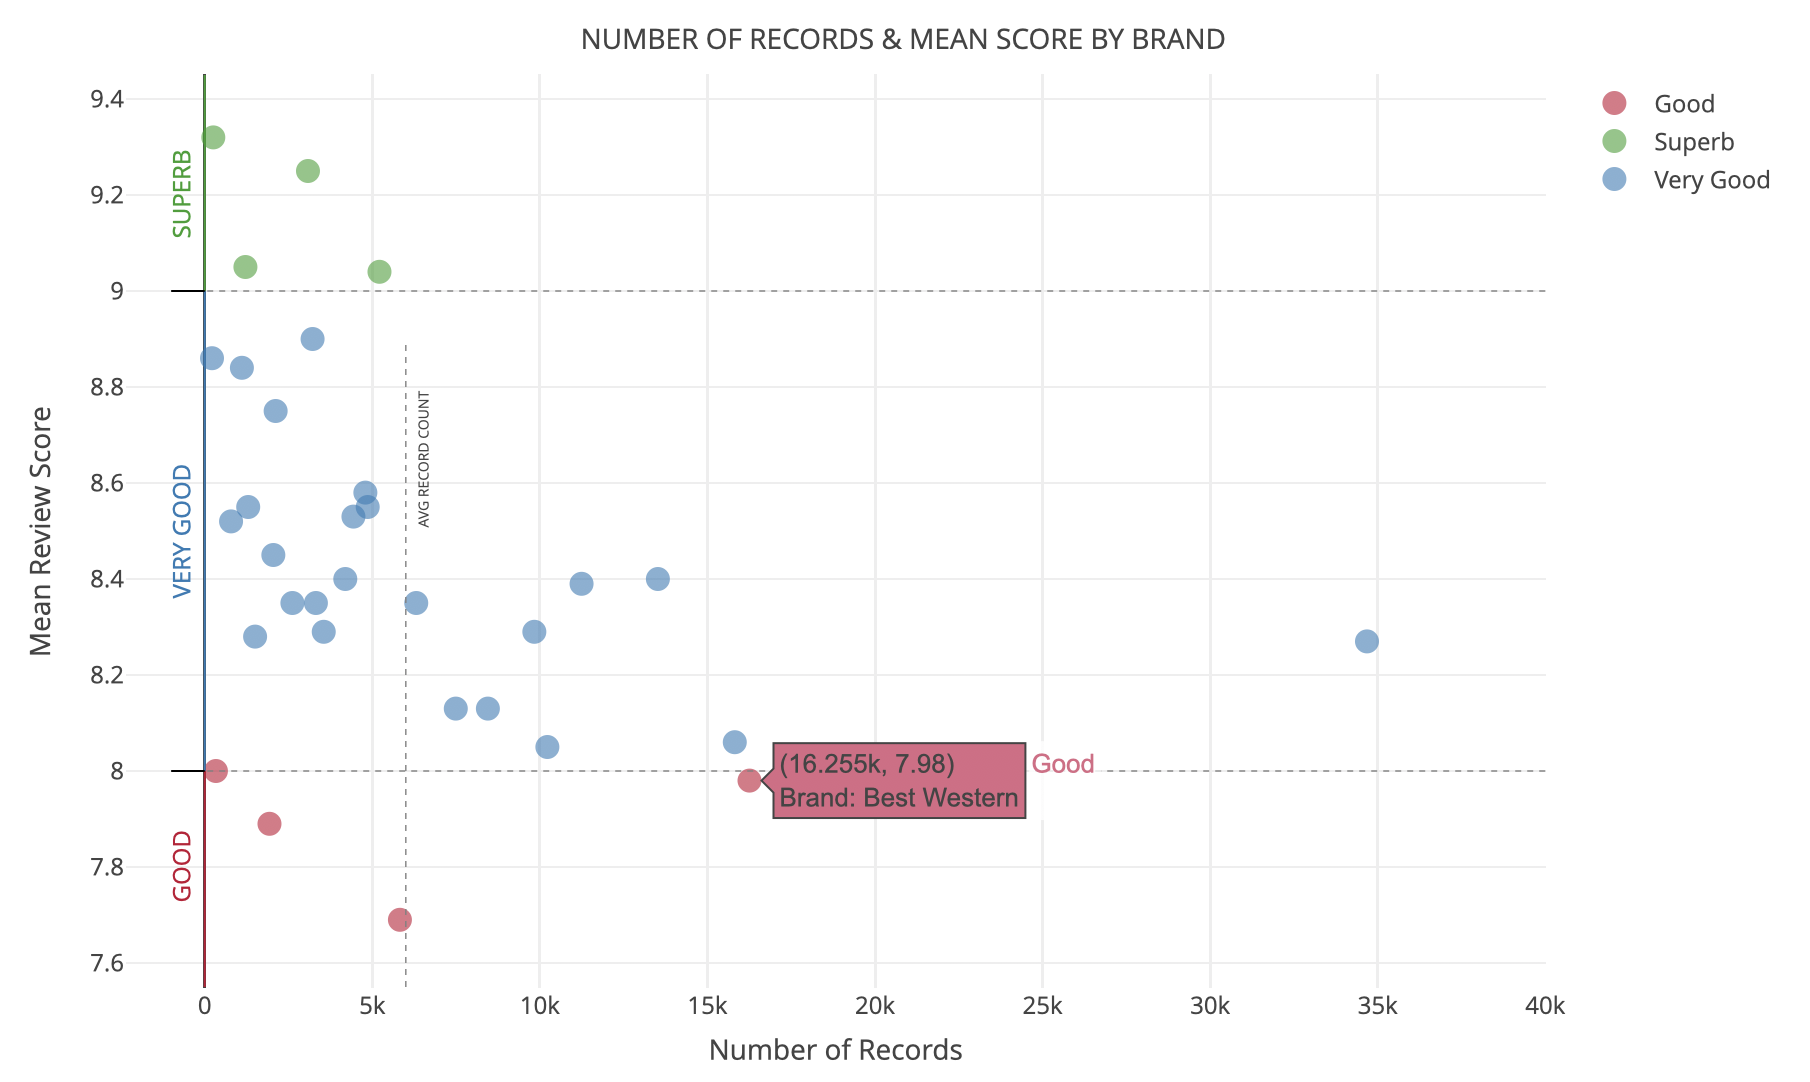
\includegraphics[width=7.2cm]{images/testimage3_1} }}%
	%	\qquad
	\subfloat[Another image ]{{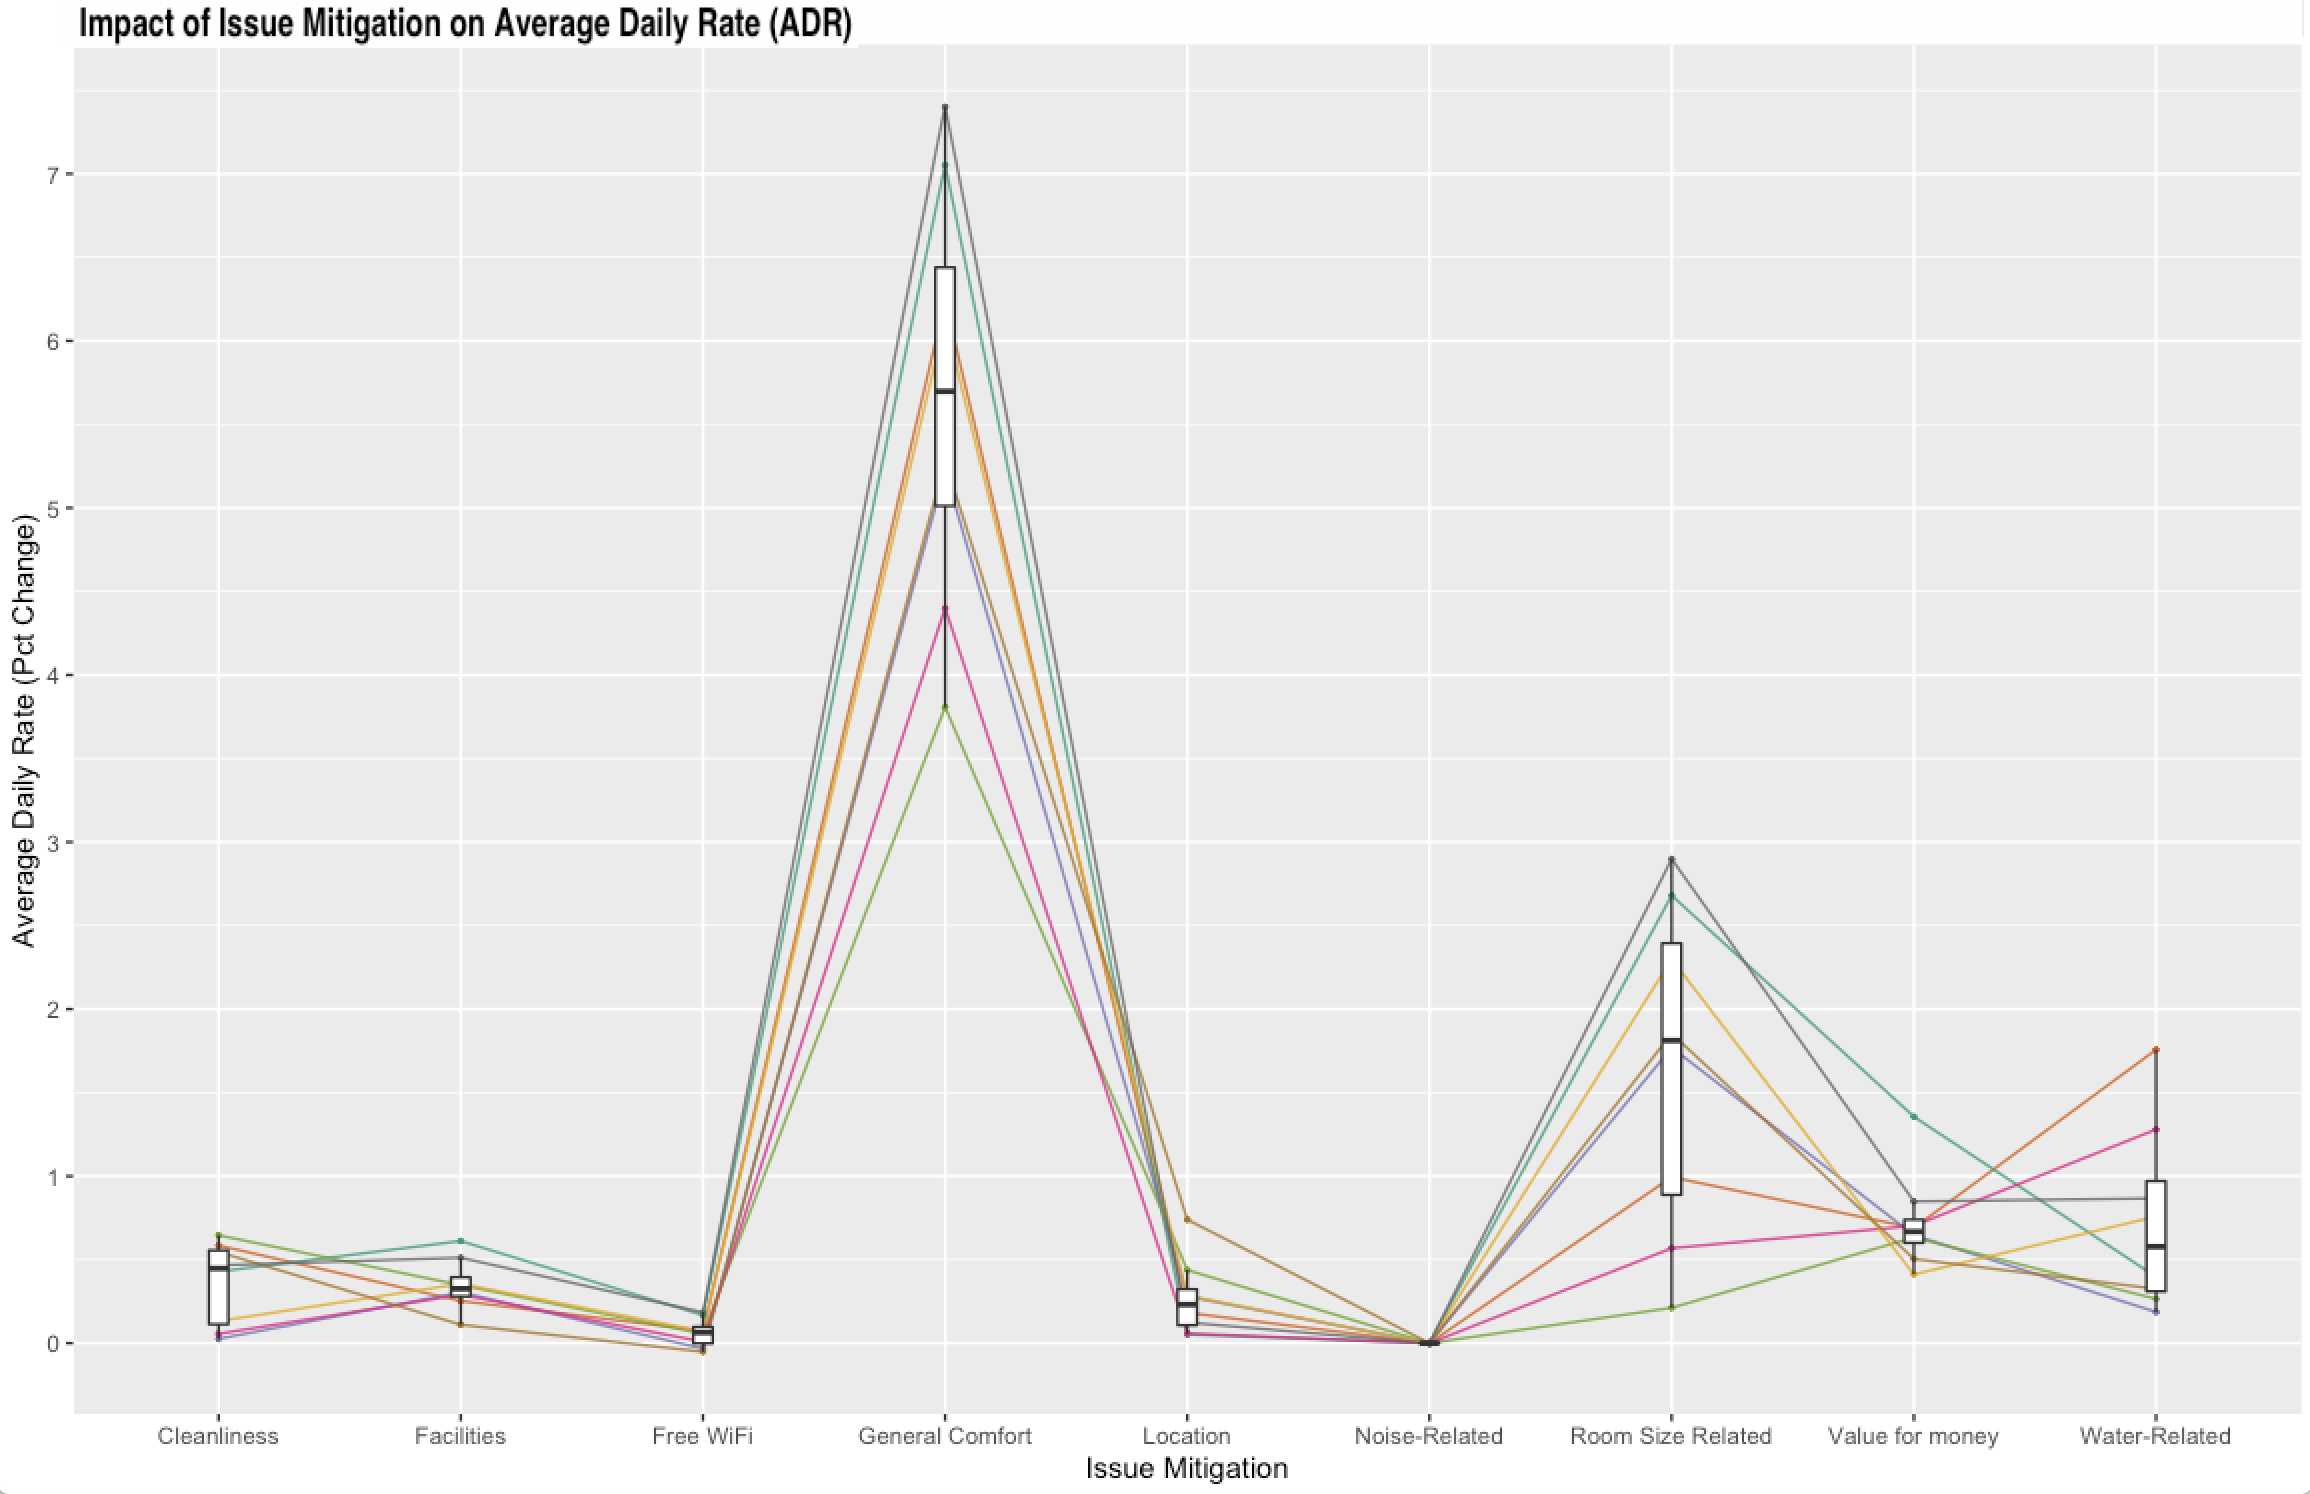
\includegraphics[width=7.2cm]{images/testimage3_2}}}%
	\caption{Floating Images}%
	\label{fig:floatimage}%
\end{figure*}


\subsection{Miscellaneous}

\subsubsection{Hyperlinks}
% HYPERLINK
\href{https://www.cnn.com}{A hyperlink to CNN.com}

% TO ADD A REFERENCE TO A SECTION
This is a section labelled as "sec1"
\label{sec:sec1}

This is a reference to the section sec1: \ref{sec:sec1}

\fbox{\begin{minipage}{43em}
		\textbf{Using fbox and minipage}\\
Text enclosed in a box
\end{minipage}}

% CODE
\subsubsection{Python Code Formatting}
\lstinputlisting[language=Python]{code/test.py}

\subsubsection{R Code Formatting}
\lstinputlisting[language=R]{code/test.R}

\subsubsection{Tables and Equations}

Examples with tables, caption centering, equations and aligned equations.

\begin{table}[!ht]
	\centering
	\captionsetup{justification=centering}
	\begin{tabular}{l|llrr}
		%		\hline
		\textbf{Model}            & \textbf{Parameter} & \textbf{Best Fit}              & \textbf{Train RMSE}             & \textbf{Test RMSE}               \\ \hline
		Linear Regression         & -                  & -                              & \rupee16,758,137 & \rupee57,778,006  \\ \hline
		Random GLM                & maxOrder           & maxInt.Order = 2        & \rupee15,551,472 & \rupee100,219,602 \\ \hline
		SVM RBF Kernel            & C, Sigma           & sigma = 26.76, C = 4     & \rupee17,075,271 & \rupee34,932,347  \\ \hline
		KNN                       & k                  & k = 5                          & \rupee12,255,888 & \rupee54,935,698  \\ \hline
		RandomForest              & mtry               & mtry = 2                       & \rupee8,724,815  & \rupee53,453,612  \\ \hline
		\rowcolor[HTML]{EFEFEF} 
		XGBoost & misc*              & max\_depth = 3, $\eta$ = 0.3, $\gamma$ = 0      & \rupee4,924,454  & \rupee65,211,901  \\ \hline
	\end{tabular}
	\caption{This is a table}
	\label{tab:state_pred}
\end{table}

Split Line in Equations
\begin{equation}
\begin{split}
\label{eqn:natsec}
ln(GVA_{Sector}) = \beta_1ln(SumOfLights)_{t}+\beta_2ln(SumElectricity)_t +\\ \beta_3ln(SumOfLightsSq)_{t} + \beta_4ln(Population)_{t} +
\alpha_i + u_{it}
\end{split}
\end{equation}

Aligned Equations
$$
\begin{aligned}
y_t &= 10.3009 -0.0042x_L - 0.0045x_B - 0.0032x_c -0.0046x_{d1} + \ldots + 0.0176x_{d6} + \eta_t \\
\eta_t &= 0.9146\eta_{t-1} + \epsilon_t -0.5015\epsilon_{t-1}\\
\epsilon_t &= \sim \text{NID}(0,0.003443)
\end{aligned}
$$

\subsubsection{Citations}
This template uses Bath BibTeX: \hyperlink{https://ctan.org/pkg/bath-bst?lang=en}{https://ctan.org/pkg/bath-bst?lang=en}

See: \hyperlink{https://github.com/alex-ball/bathbib/tree/master/bst}{https://github.com/alex-ball/bathbib/tree/master/bst}

This is a citation \citep{Elvidge_Baugh_Zhizhin_Hsu_Ghosh_2017} using \texttt{citep}.

This is a citation \cite{Tibshirani_1996} using \texttt{cite}

\pagebreak
\end{verbatim}
{\color{red} \rule{\linewidth}{0.5mm}}

\textcolor{red}{\textbf{FONT USAGE}}

The Arial font is recommended for the Individual Research Report. However, this needs to be installed manually as discussed in this document. For Overleaf, Helvetica has been used. If you are able to install Arial, comment the line \texttt{usepackage[scaled]\{helvet\}} and uncomment \texttt{usepackage\{uarial\}}.

{\color{red} \rule{\linewidth}{0.5mm}}

\textbf{FORMATTING AND PAGE NUMBERING CONVENTIONS USED}

\begin{itemize}
	\item Geometry
	\begin{itemize}
		\item left-hand margin of 4 cm;
		\item right-hand margin of 2.5cm (1 inch);
		\item top margin 2.5cm (1 inch);
		\item bottom margin 2.5cm (1 inch).
	\end{itemize}
	\begin{itemize}
		\item The Synopsis, Acknowledgements, List of Contents and Notation should be numbered with upper case Roman Numerals.
		\item The main text, starting with the first page of the first chapter (or Introduction) should be numbered, starting with page 1, using Arabic Numerals, through to the end of the references.
		\item \textbf{Appendices should be numbered using lower case Roman Numerals. -- Check to make sure this is what is needed. If not comment \texttt{\\pagenumbering\{roman\}} in template before Appendix}
	\end{itemize}
	\item Pages must be numbered at the bottom centre of the page.
	\item The title page should be blank.
\end{itemize}

\subsection{Prerequisites}

There are 2 primary pre-requisites: First, to install the Bath BibTeX style and second to install the Arial font. Note that if Arial cannot be installed, it may be possible to use Helvetica if the department agrees 

\textbf{1. Install the Bath BibTeX style (See Included Folder)}

\textbf{2. Install Font Arial}: See \hyperlink{https://www.tug.org/fonts/getnonfreefonts/}{https://www.tug.org/fonts/getnonfreefonts/} and 

\textbf{Notes from \hyperlink{https://tex.stackexchange.com/questions/37120/how-can-i-install-uarial-sty-on-a-mac}{Install uarial on a Mac} question on Stackexchange: }

The font can be easily installed via the script getnonfreefonts. It is available at tug.org: \hyperlink{http://www.tug.org/fonts/getnonfreefonts/}{getnonfreefonts}. I tried the installation of \hyperlink{http://www.tug.org/fonts/getnonfreefonts/install-getnonfreefonts}{getnonfreefonts} on my Mac.

\begin{itemize}
	\item Install MacTeX 
	\item Download the installation script. Open the terminal and go to the folder Download
	
	\texttt{cd Download}
	\item Run the installation: \texttt{sudo texlua install-getnonfreefonts}
	
	The installation finished and the scipts with their execute files getnonefreefonts and getnonfreefonts-sys are now located at \texttt{/usr/local/texlive/2011/bin/x86\_64-darwin/}
	
	\item Now you can run the script \texttt{sudo getnonfreefonts-sys -a}
\end{itemize}

\subsection{Images}
\begin{figure*}[!ht]
	\centering
	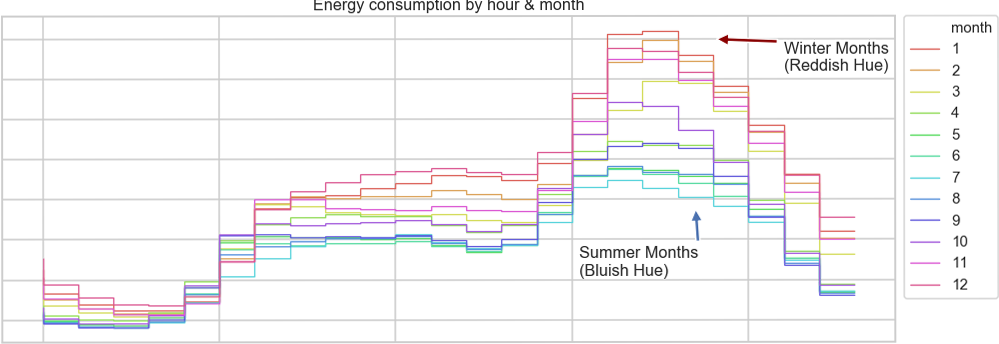
\includegraphics[width=16cm]{images/testimage1}
	\caption{This is an image}
	\label{fig:testimage1}
\end{figure*}

\begin{figure*}[!ht]
	\centering
	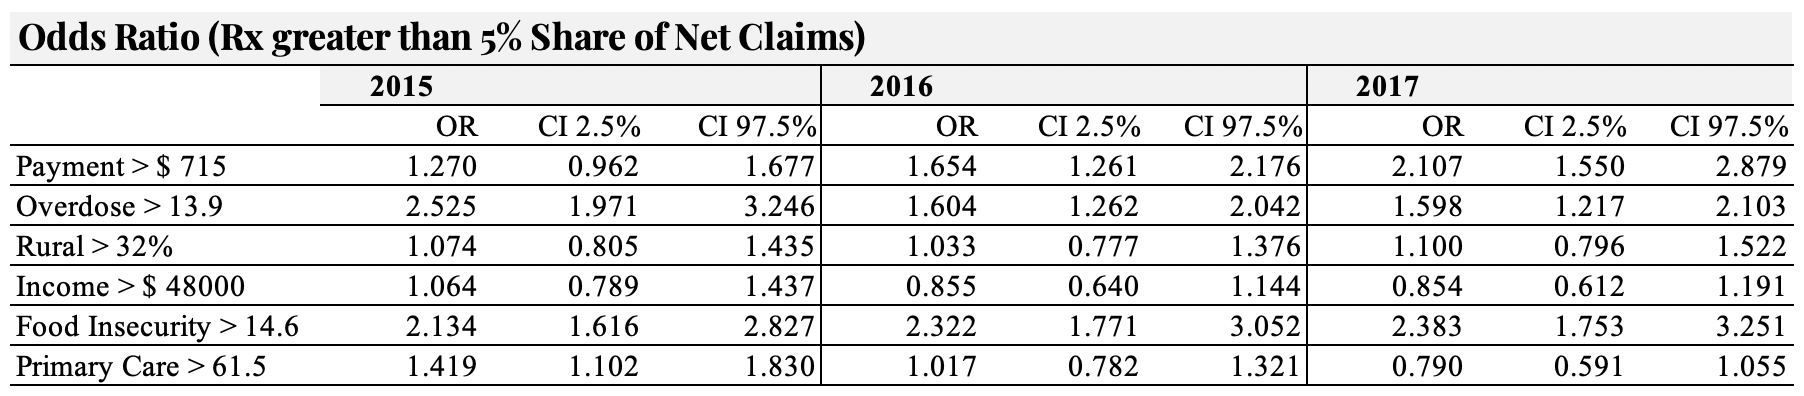
\includegraphics[width=16cm]{images/testimage2}
	%	\caption{Round 1 Blue Strategy to increase Market Share}
	\captionof{table}[This is a table shown as an image]{This is a table shown as an image}
	\label{fig:testimage2}
\end{figure*}

\begin{figure*}[!ht]
	\centering
	\subfloat[A floating image]{{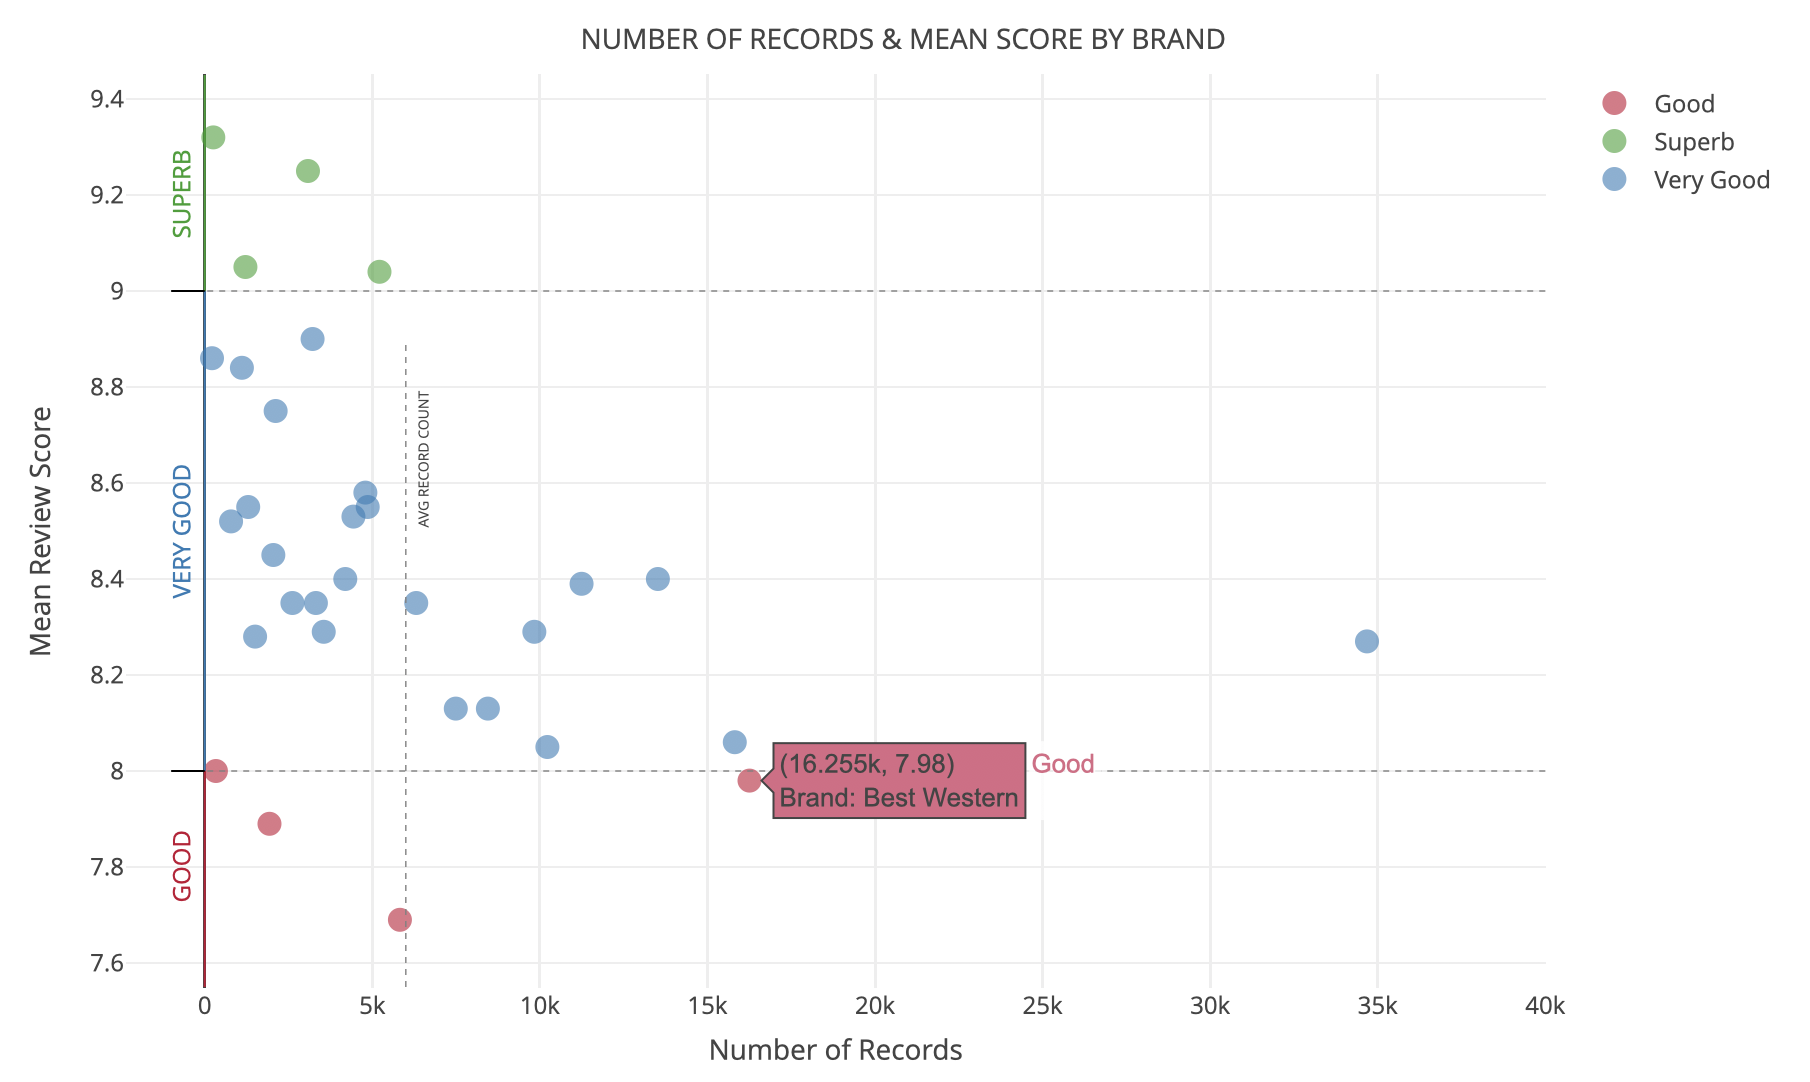
\includegraphics[width=7.2cm]{images/testimage3_1} }}%
	%	\qquad
	\subfloat[Another image ]{{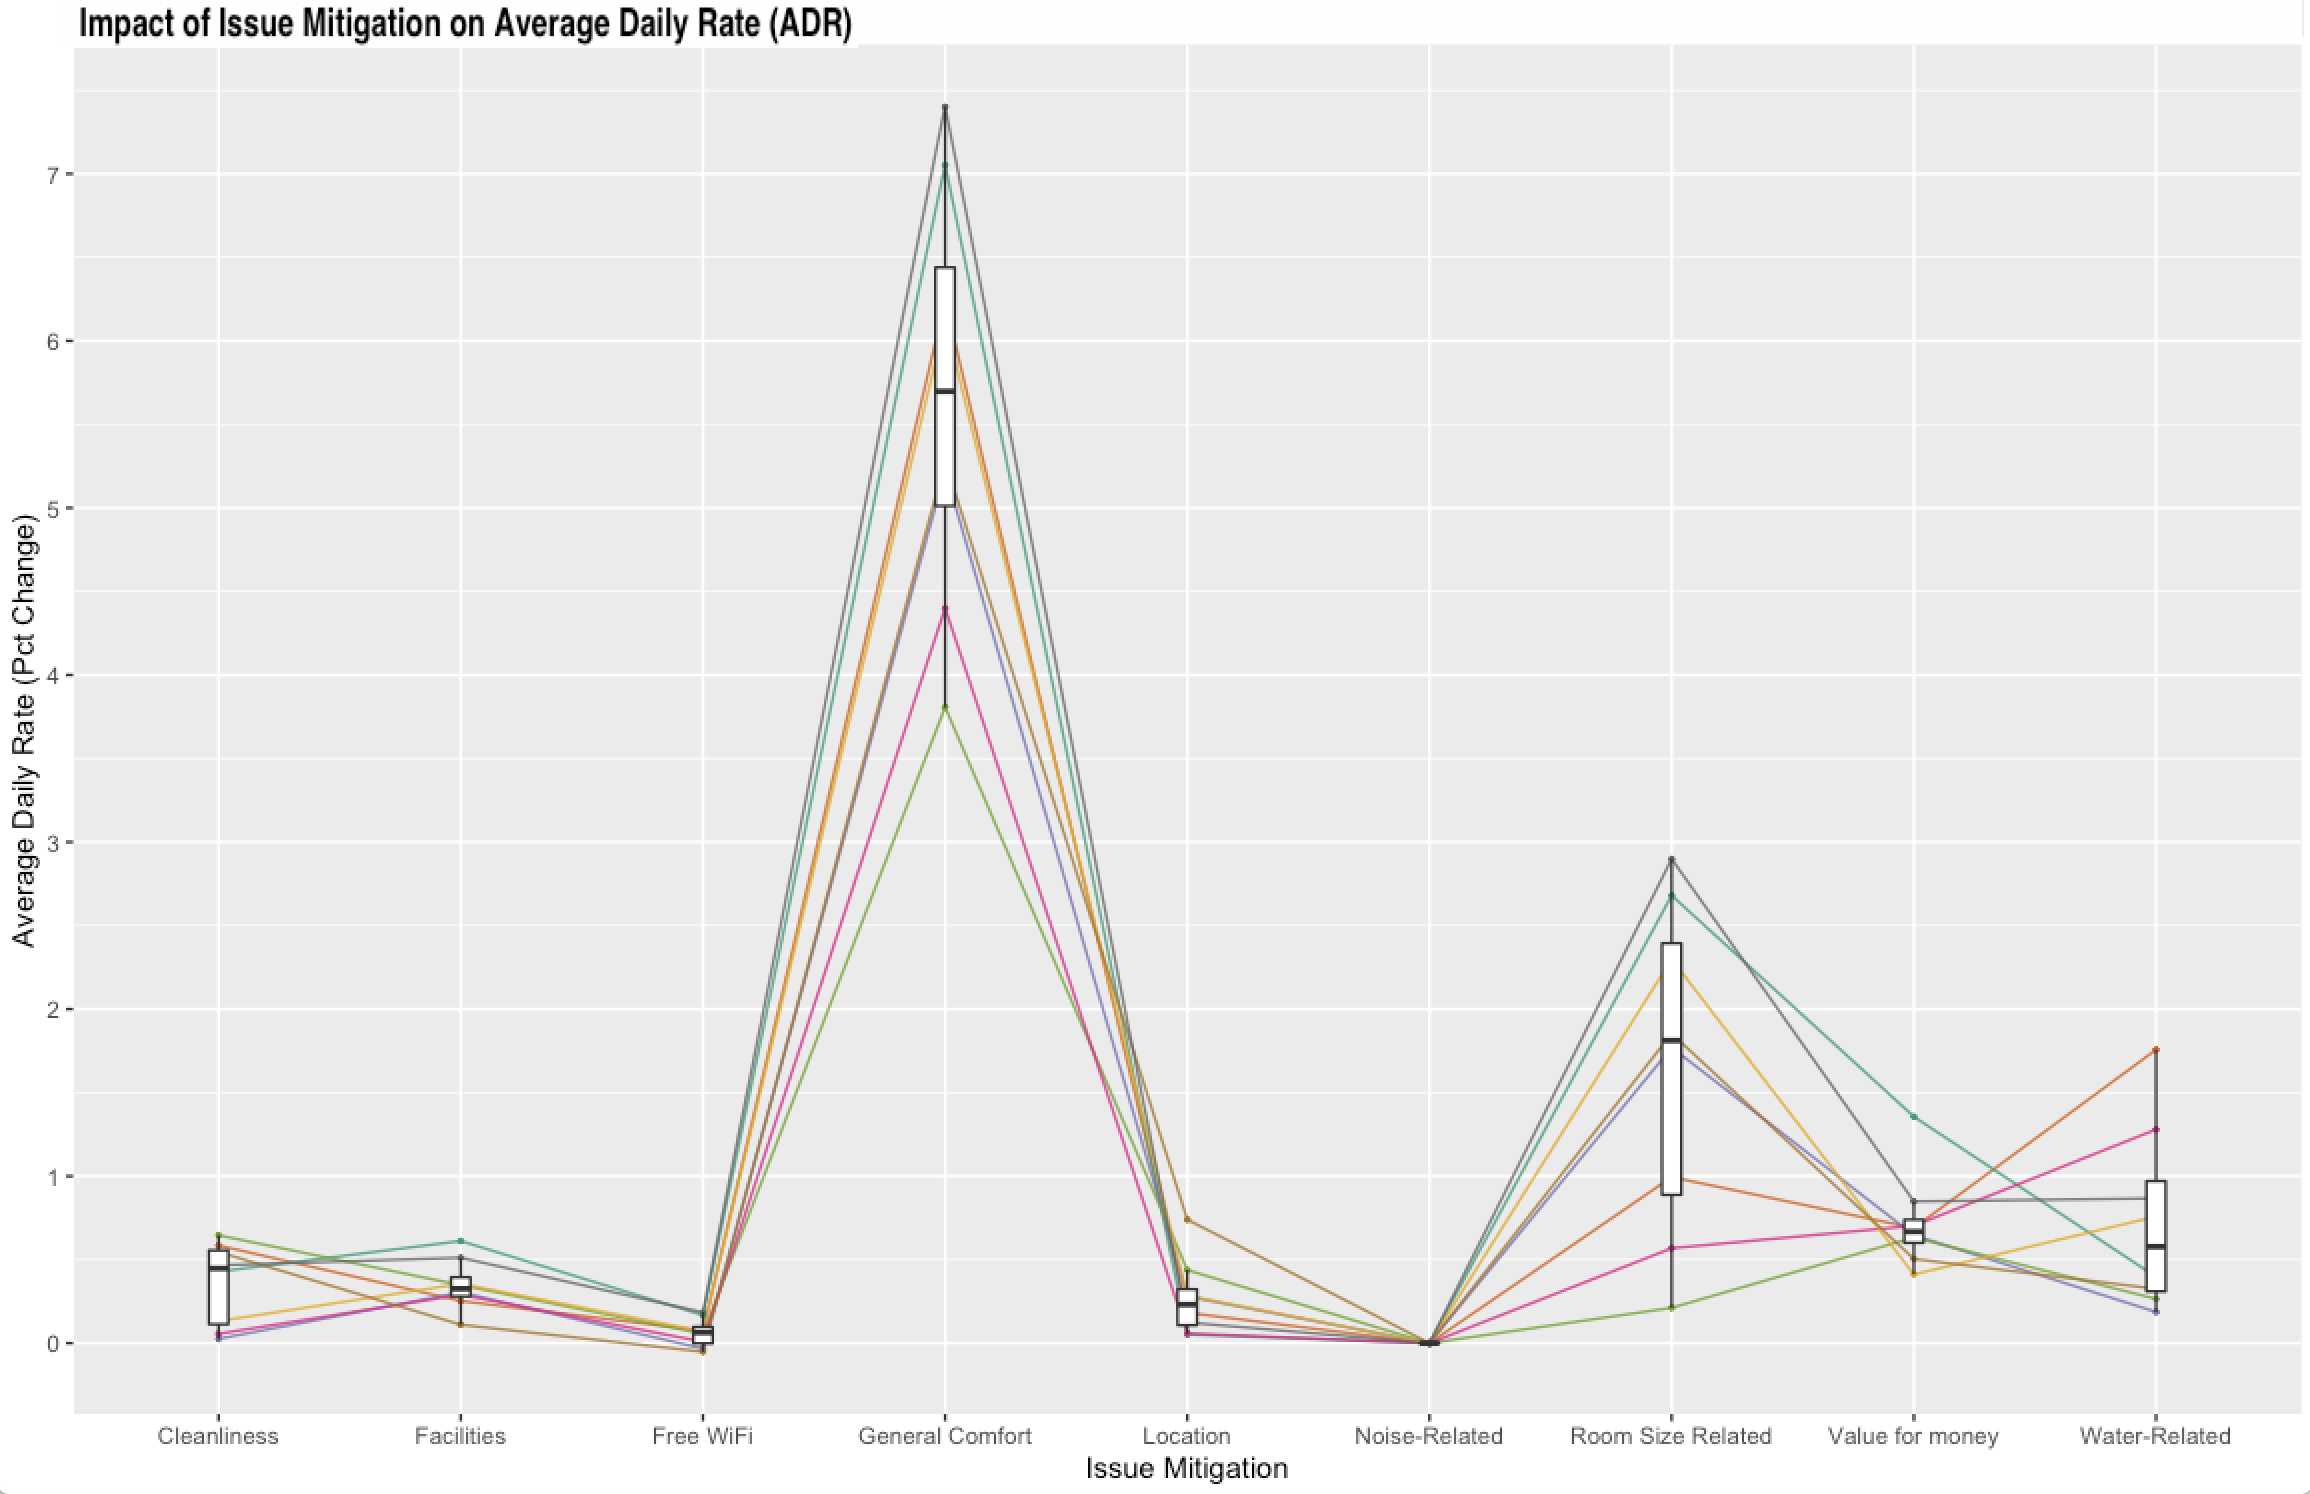
\includegraphics[width=7.2cm]{images/testimage3_2}}}%
	\caption{Floating Images}%
	\label{fig:floatimage}%
\end{figure*}


\subsection{Miscellaneous}

\subsubsection{Hyperlinks}
% HYPERLINK
\href{https://www.cnn.com}{A hyperlink to CNN.com}

% TO ADD A REFERENCE TO A SECTION
This is a section labelled as "sec1"
\label{sec:sec1}

This is a reference to the section sec1: \ref{sec:sec1}

\fbox{\begin{minipage}{43em}
		\textbf{Using fbox and minipage}\\
Text enclosed in a box
\end{minipage}}

% CODE
\subsubsection{Python Code Formatting}
\lstinputlisting[language=Python]{code/test.py}

\subsubsection{R Code Formatting}
\lstinputlisting[language=R]{code/test.R}

\subsubsection{Tables and Equations}

Examples with tables, caption centering, equations and aligned equations.

\begin{table}[!ht]
	\centering
	\captionsetup{justification=centering}
	\begin{tabular}{l|llrr}
		%		\hline
		\textbf{Model}            & \textbf{Parameter} & \textbf{Best Fit}              & \textbf{Train RMSE}             & \textbf{Test RMSE}               \\ \hline
		Linear Regression         & -                  & -                              & \rupee16,758,137 & \rupee57,778,006  \\ \hline
		Random GLM                & maxOrder           & maxInt.Order = 2        & \rupee15,551,472 & \rupee100,219,602 \\ \hline
		SVM RBF Kernel            & C, Sigma           & sigma = 26.76, C = 4     & \rupee17,075,271 & \rupee34,932,347  \\ \hline
		KNN                       & k                  & k = 5                          & \rupee12,255,888 & \rupee54,935,698  \\ \hline
		RandomForest              & mtry               & mtry = 2                       & \rupee8,724,815  & \rupee53,453,612  \\ \hline
		\rowcolor[HTML]{EFEFEF} 
		XGBoost & misc*              & max\_depth = 3, $\eta$ = 0.3, $\gamma$ = 0      & \rupee4,924,454  & \rupee65,211,901  \\ \hline
	\end{tabular}
	\caption{This is a table}
	\label{tab:state_pred}
\end{table}

Split Line in Equations
\begin{equation}
\begin{split}
\label{eqn:natsec}
ln(GVA_{Sector}) = \beta_1ln(SumOfLights)_{t}+\beta_2ln(SumElectricity)_t +\\ \beta_3ln(SumOfLightsSq)_{t} + \beta_4ln(Population)_{t} +
\alpha_i + u_{it}
\end{split}
\end{equation}

Aligned Equations
$$
\begin{aligned}
y_t &= 10.3009 -0.0042x_L - 0.0045x_B - 0.0032x_c -0.0046x_{d1} + \ldots + 0.0176x_{d6} + \eta_t \\
\eta_t &= 0.9146\eta_{t-1} + \epsilon_t -0.5015\epsilon_{t-1}\\
\epsilon_t &= \sim \text{NID}(0,0.003443)
\end{aligned}
$$

\subsubsection{Citations}
This template uses Bath BibTeX: \hyperlink{https://ctan.org/pkg/bath-bst?lang=en}{https://ctan.org/pkg/bath-bst?lang=en}

See: \hyperlink{https://github.com/alex-ball/bathbib/tree/master/bst}{https://github.com/alex-ball/bathbib/tree/master/bst}

This is a citation \citep{Elvidge_Baugh_Zhizhin_Hsu_Ghosh_2017} using \texttt{citep}.

This is a citation \cite{Tibshirani_1996} using \texttt{cite}

\pagebreak
\end{verbatim}
{\color{red} \rule{\linewidth}{0.5mm}}

\textcolor{red}{\textbf{FONT USAGE}}

The Arial font is recommended for the Individual Research Report. However, this needs to be installed manually as discussed in this document. For Overleaf, Helvetica has been used. If you are able to install Arial, comment the line \texttt{usepackage[scaled]\{helvet\}} and uncomment \texttt{usepackage\{uarial\}}.

{\color{red} \rule{\linewidth}{0.5mm}}

\textbf{FORMATTING AND PAGE NUMBERING CONVENTIONS USED}

\begin{itemize}
	\item Geometry
	\begin{itemize}
		\item left-hand margin of 4 cm;
		\item right-hand margin of 2.5cm (1 inch);
		\item top margin 2.5cm (1 inch);
		\item bottom margin 2.5cm (1 inch).
	\end{itemize}
	\begin{itemize}
		\item The Synopsis, Acknowledgements, List of Contents and Notation should be numbered with upper case Roman Numerals.
		\item The main text, starting with the first page of the first chapter (or Introduction) should be numbered, starting with page 1, using Arabic Numerals, through to the end of the references.
		\item \textbf{Appendices should be numbered using lower case Roman Numerals. -- Check to make sure this is what is needed. If not comment \texttt{\\pagenumbering\{roman\}} in template before Appendix}
	\end{itemize}
	\item Pages must be numbered at the bottom centre of the page.
	\item The title page should be blank.
\end{itemize}

\subsection{Prerequisites}

There are 2 primary pre-requisites: First, to install the Bath BibTeX style and second to install the Arial font. Note that if Arial cannot be installed, it may be possible to use Helvetica if the department agrees 

\textbf{1. Install the Bath BibTeX style (See Included Folder)}

\textbf{2. Install Font Arial}: See \hyperlink{https://www.tug.org/fonts/getnonfreefonts/}{https://www.tug.org/fonts/getnonfreefonts/} and 

\textbf{Notes from \hyperlink{https://tex.stackexchange.com/questions/37120/how-can-i-install-uarial-sty-on-a-mac}{Install uarial on a Mac} question on Stackexchange: }

The font can be easily installed via the script getnonfreefonts. It is available at tug.org: \hyperlink{http://www.tug.org/fonts/getnonfreefonts/}{getnonfreefonts}. I tried the installation of \hyperlink{http://www.tug.org/fonts/getnonfreefonts/install-getnonfreefonts}{getnonfreefonts} on my Mac.

\begin{itemize}
	\item Install MacTeX 
	\item Download the installation script. Open the terminal and go to the folder Download
	
	\texttt{cd Download}
	\item Run the installation: \texttt{sudo texlua install-getnonfreefonts}
	
	The installation finished and the scipts with their execute files getnonefreefonts and getnonfreefonts-sys are now located at \texttt{/usr/local/texlive/2011/bin/x86\_64-darwin/}
	
	\item Now you can run the script \texttt{sudo getnonfreefonts-sys -a}
\end{itemize}

\subsection{Images}
\begin{figure*}[!ht]
	\centering
	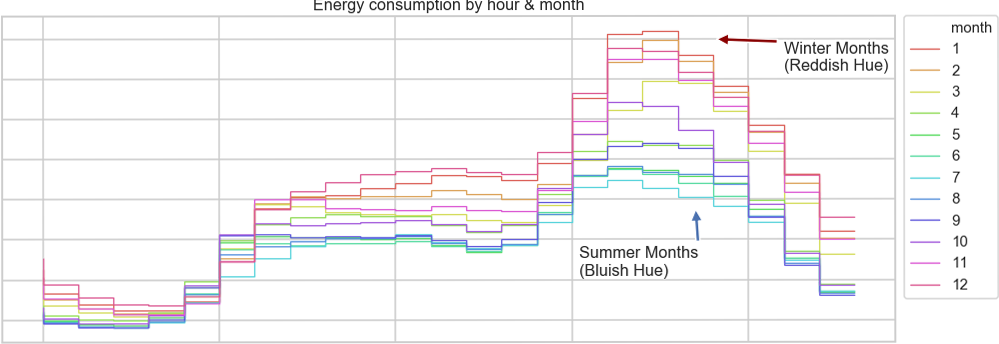
\includegraphics[width=16cm]{images/testimage1}
	\caption{This is an image}
	\label{fig:testimage1}
\end{figure*}

\begin{figure*}[!ht]
	\centering
	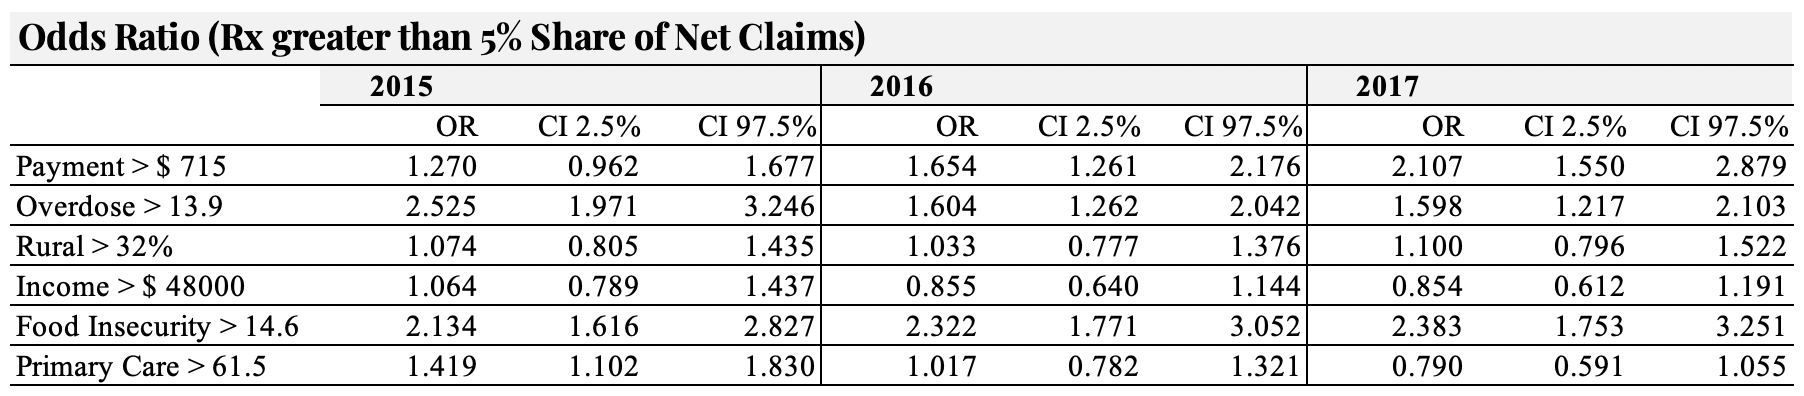
\includegraphics[width=16cm]{images/testimage2}
	%	\caption{Round 1 Blue Strategy to increase Market Share}
	\captionof{table}[This is a table shown as an image]{This is a table shown as an image}
	\label{fig:testimage2}
\end{figure*}

\begin{figure*}[!ht]
	\centering
	\subfloat[A floating image]{{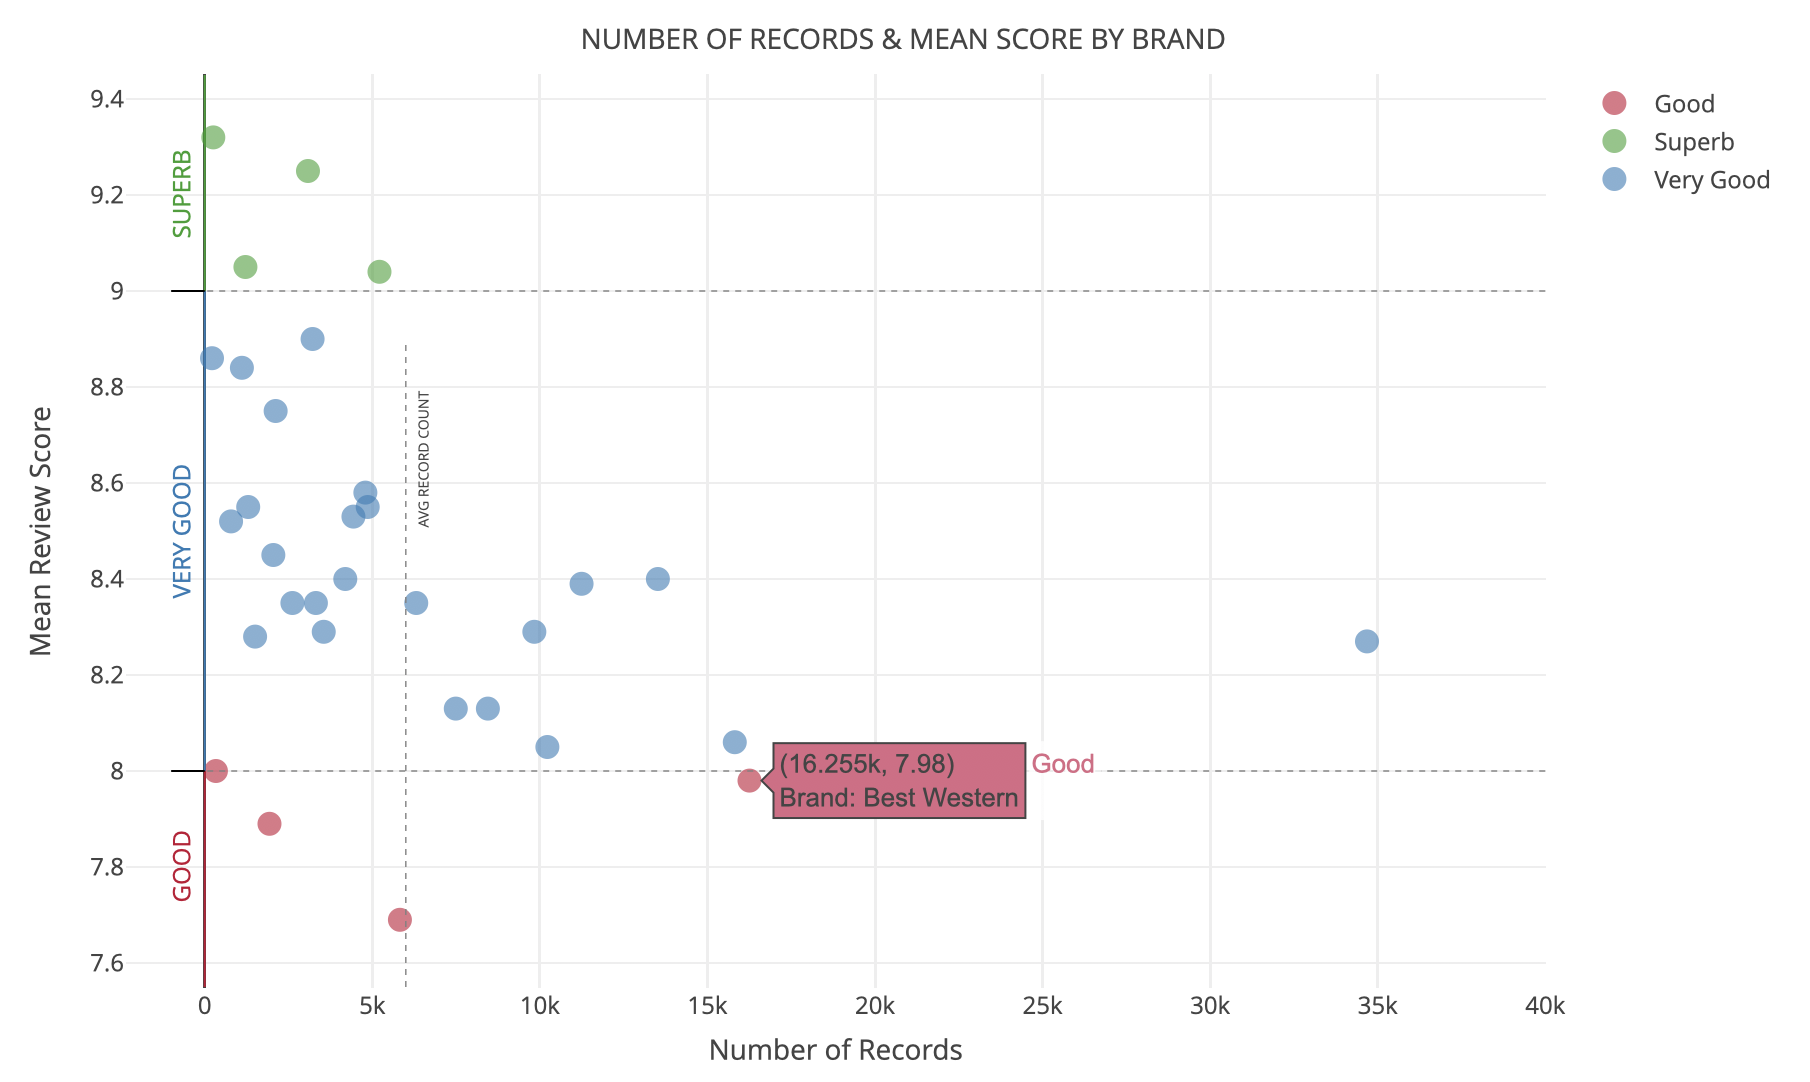
\includegraphics[width=7.2cm]{images/testimage3_1} }}%
	%	\qquad
	\subfloat[Another image ]{{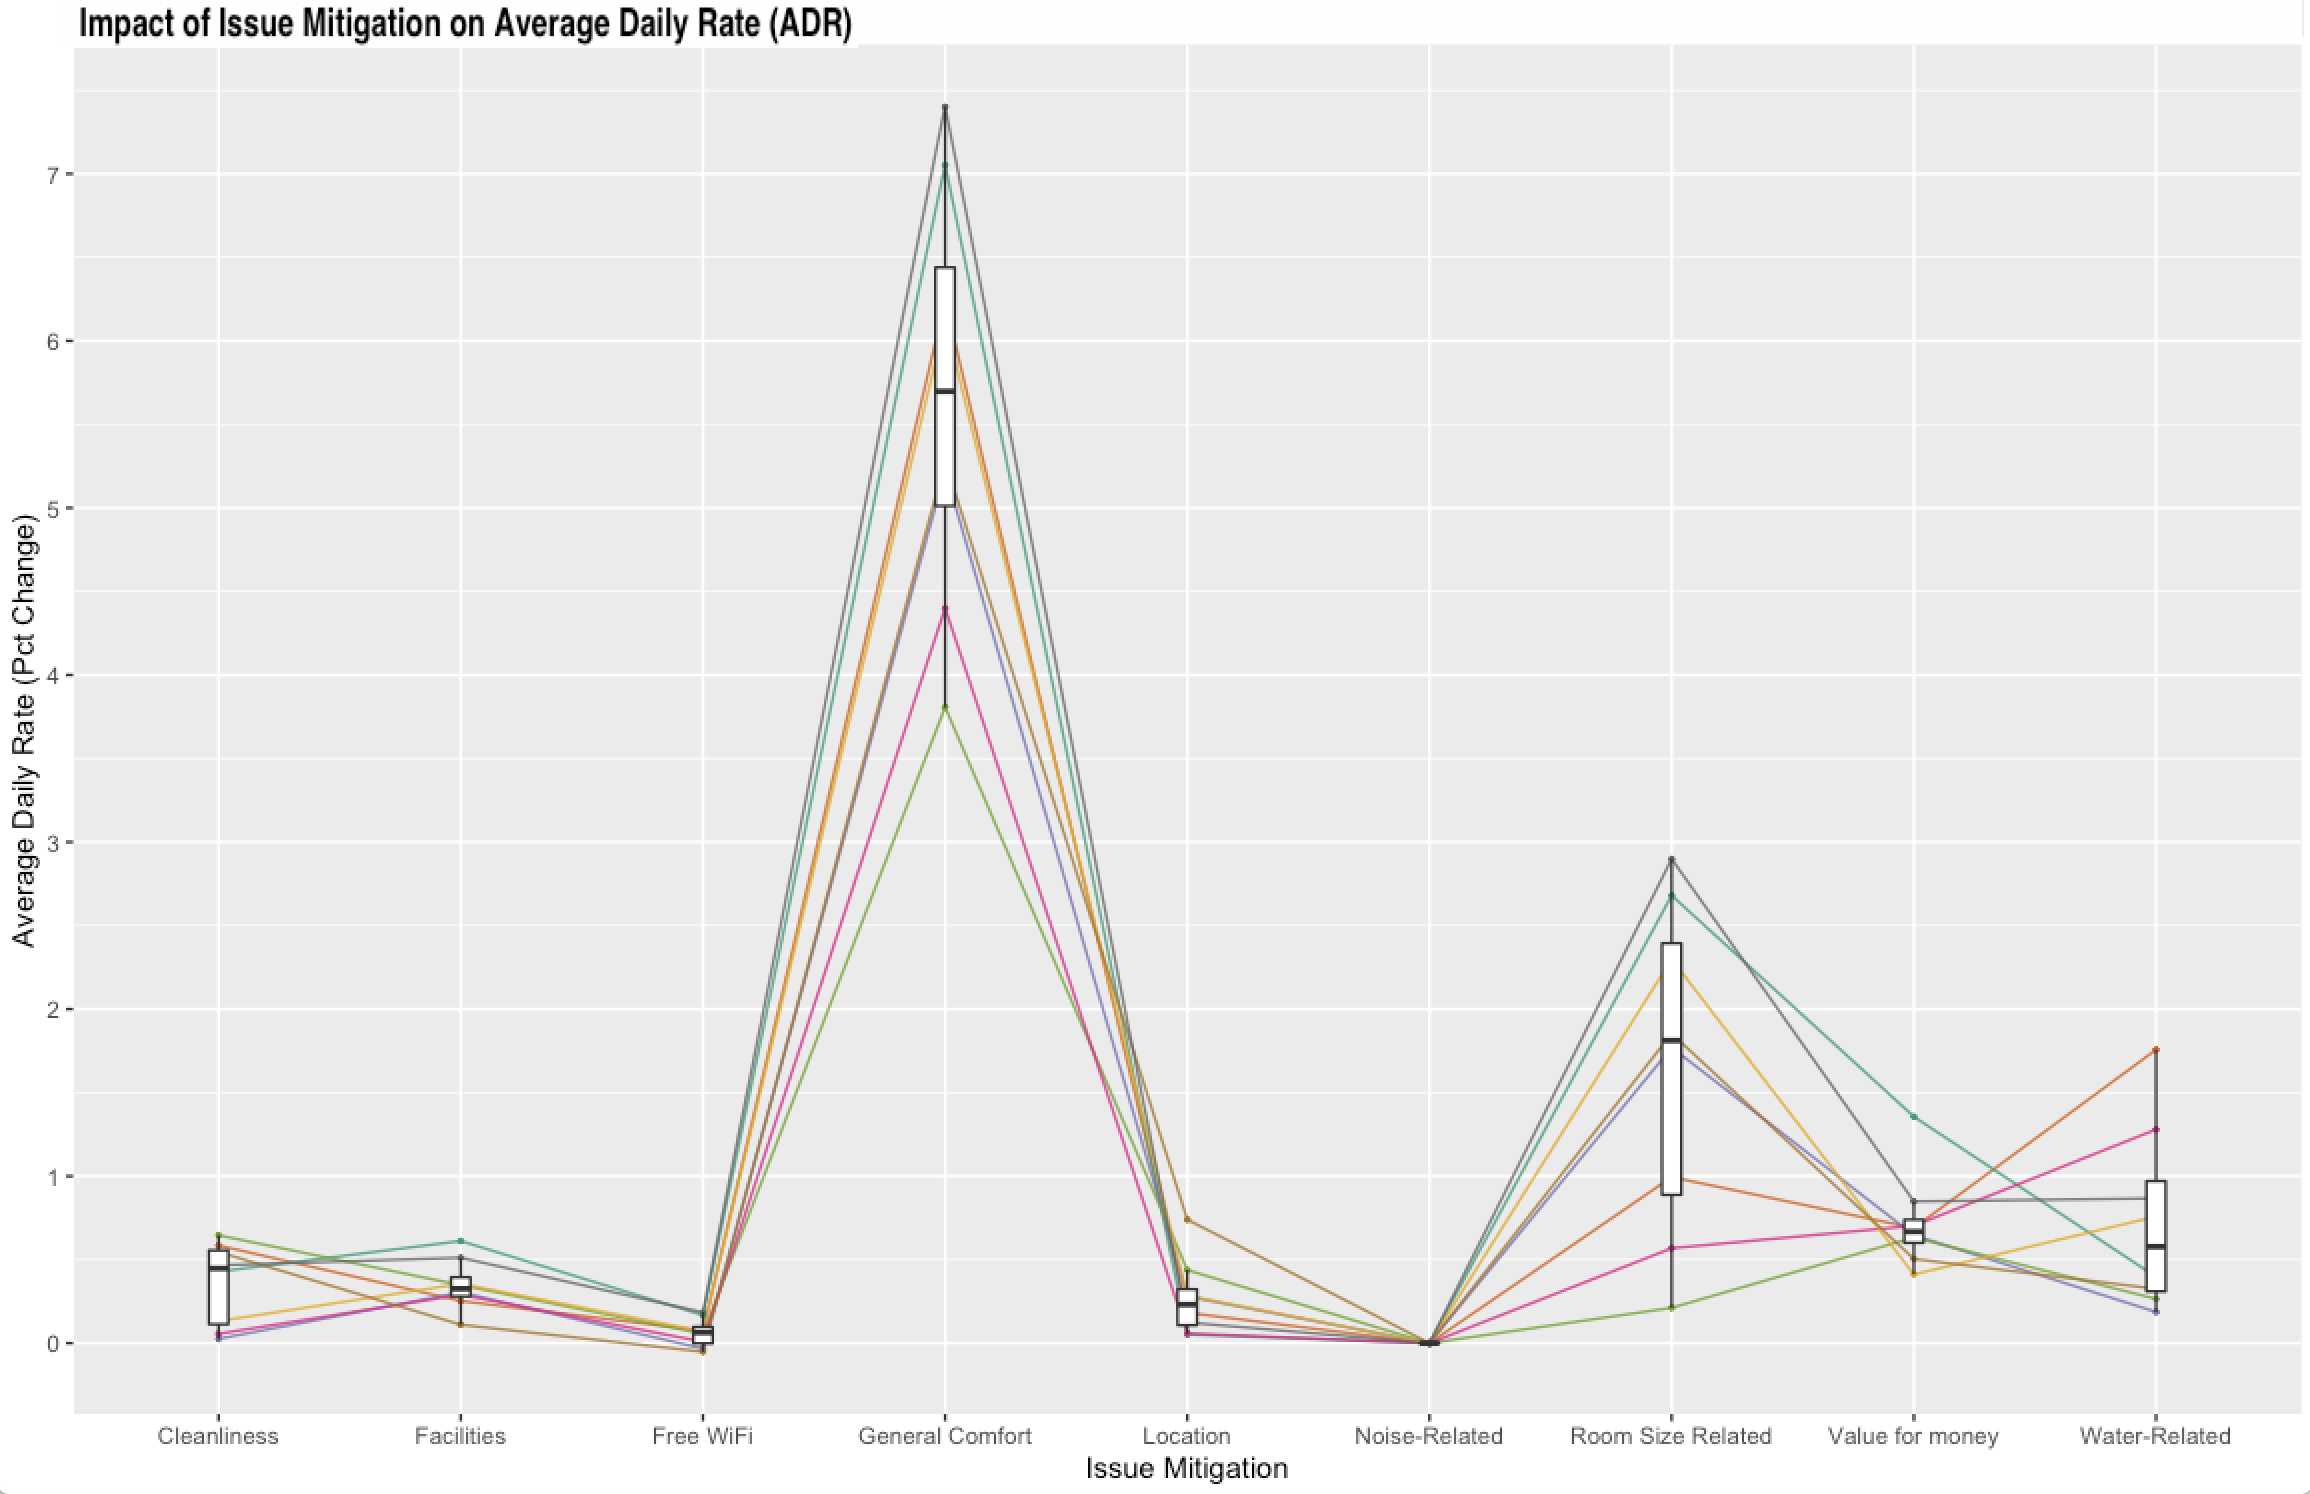
\includegraphics[width=7.2cm]{images/testimage3_2}}}%
	\caption{Floating Images}%
	\label{fig:floatimage}%
\end{figure*}


\subsection{Miscellaneous}

\subsubsection{Hyperlinks}
% HYPERLINK
\href{https://www.cnn.com}{A hyperlink to CNN.com}

% TO ADD A REFERENCE TO A SECTION
This is a section labelled as "sec1"
\label{sec:sec1}

This is a reference to the section sec1: \ref{sec:sec1}

\fbox{\begin{minipage}{43em}
		\textbf{Using fbox and minipage}\\
Text enclosed in a box
\end{minipage}}

% CODE
\subsubsection{Python Code Formatting}
\lstinputlisting[language=Python]{code/test.py}

\subsubsection{R Code Formatting}
\lstinputlisting[language=R]{code/test.R}

\subsubsection{Tables and Equations}

Examples with tables, caption centering, equations and aligned equations.

\begin{table}[!ht]
	\centering
	\captionsetup{justification=centering}
	\begin{tabular}{l|llrr}
		%		\hline
		\textbf{Model}            & \textbf{Parameter} & \textbf{Best Fit}              & \textbf{Train RMSE}             & \textbf{Test RMSE}               \\ \hline
		Linear Regression         & -                  & -                              & \rupee16,758,137 & \rupee57,778,006  \\ \hline
		Random GLM                & maxOrder           & maxInt.Order = 2        & \rupee15,551,472 & \rupee100,219,602 \\ \hline
		SVM RBF Kernel            & C, Sigma           & sigma = 26.76, C = 4     & \rupee17,075,271 & \rupee34,932,347  \\ \hline
		KNN                       & k                  & k = 5                          & \rupee12,255,888 & \rupee54,935,698  \\ \hline
		RandomForest              & mtry               & mtry = 2                       & \rupee8,724,815  & \rupee53,453,612  \\ \hline
		\rowcolor[HTML]{EFEFEF} 
		XGBoost & misc*              & max\_depth = 3, $\eta$ = 0.3, $\gamma$ = 0      & \rupee4,924,454  & \rupee65,211,901  \\ \hline
	\end{tabular}
	\caption{This is a table}
	\label{tab:state_pred}
\end{table}

Split Line in Equations
\begin{equation}
\begin{split}
\label{eqn:natsec}
ln(GVA_{Sector}) = \beta_1ln(SumOfLights)_{t}+\beta_2ln(SumElectricity)_t +\\ \beta_3ln(SumOfLightsSq)_{t} + \beta_4ln(Population)_{t} +
\alpha_i + u_{it}
\end{split}
\end{equation}

Aligned Equations
$$
\begin{aligned}
y_t &= 10.3009 -0.0042x_L - 0.0045x_B - 0.0032x_c -0.0046x_{d1} + \ldots + 0.0176x_{d6} + \eta_t \\
\eta_t &= 0.9146\eta_{t-1} + \epsilon_t -0.5015\epsilon_{t-1}\\
\epsilon_t &= \sim \text{NID}(0,0.003443)
\end{aligned}
$$

\subsubsection{Citations}
This template uses Bath BibTeX: \hyperlink{https://ctan.org/pkg/bath-bst?lang=en}{https://ctan.org/pkg/bath-bst?lang=en}

See: \hyperlink{https://github.com/alex-ball/bathbib/tree/master/bst}{https://github.com/alex-ball/bathbib/tree/master/bst}

This is a citation \citep{Elvidge_Baugh_Zhizhin_Hsu_Ghosh_2017} using \texttt{citep}.

This is a citation \cite{Tibshirani_1996} using \texttt{cite}

\pagebreak

\section*{Synopsis}
\textbf{MAXIMUM 250 WORDS}
All Reports must include a one page synopsis. This should include a clear statement that sets out the terms of reference and objectives of the Report as agreed with the Supervisor.
%\include{synopsis.tex}


\pagebreak

\section*{Acknowledgments}
%\include{Acknowledgments.tex}
\blindtext
\pagebreak

\section*{Notation}
The extent to which you list any symbols used in your report must be left to your discretion. Symbols, which are used in several parts of your report, should preferably be listed before the main text for easy reference. Symbols which are used only once or in one part of the report may be referred to in that part only. Generally, try to place yourself in the position of a reader with average background knowledge and arrange the notation in a manner which will be most convenient for him/her to follow.
\pagebreak

%\section*{List of Contents}
\tableofcontents
\pagebreak
\listoffigures
\listoftables
\pagebreak
\newpage
%\section{Notation}
%\textbf{IF APPLICABLE}
%%\include{Acknowledgments.tex}


\cleardoublepage\pagenumbering{arabic}

\section{Introduction}
\textbf{Introduction, background to research, overview of research, aims and objectives, terms of reference, key research questions}

\begin{itemize}
	\item The Main Text area is the section that contains your fully formed thesis and it is the section where the 8,000-word limit applies.
	Your Report, irrespective of the nature of the topic, must contain critical comment based on the considered assessment of the material/evidence presented in it: this is an essential requirement, as are the conclusions of the report.
	\item Your Report will not be made available to the general public by any means of distribution and, accordingly, you do not need to worry about getting permission from copyright holders in making direct quotations or copying figures from other publications. However, your sources must be acknowledged. You must also indicate by the use of inverted commas or different typeface the quoted material so that it is clearly identified as such. However, if you subsequently write up your work, in conjunction with your Supervisor, as a paper, then you are subject to normal copyright laws and must only quote very brief extracts even from those Journals, which subscribe to the Royal Society's convention on Fair Copying.
	\item Depending on the nature of the report, the main text should start with a review of previous literature. In a review and discussion of the work of others (and at all times) it should be clear from the text which of the opinions expressed are those of the author and which are those of other people.
	\item Where appropriate, students can include links to electronic/video material created in support of and as part of the IRR.
	
	
	
\end{itemize}

Your final Report should be no longer than 8,000 words. The word limit applies to the main text area only, as this is where your report is introduced and then carried forward. Your final word-count should not include: title page, synopsis, acknowledgements, list of contents, notation (if applicable), references, bibliography or appendix/appendices. Shorter Reports are allowed depending on the nature of the research (for example some mathematical and statistical projects are usually shorter than qualitative projects). Reports longer than 8,000 words will be penalised.\\
\\
If the Report is to contain a considerable number of tables and figures, it may be best to place them in an appendix and use in the main text only such summary tables or charts as will assist the reader in following your arguments without necessarily having to go into great detail. This may help to ensure a smooth and uninterrupted presentation.\\
\\
5.11 UNACCEPTABLE PRESENTATION
\textbf{Examiners will not accept projects where the presentational guidelines are not adhered to}. They will not accept projects that have any of the following:
Copyright statements (in any format including as a header/footer);
Confidentiality statements (in any format including as a header/footer);
Non standard font size, type and line spacing;
Page numbers missing;
No contents pages or contents pages with no page numbers indicated.



\pagebreak

\section{Literature Review}
\subsection{Literature Subsection}
\blindtext
\pagebreak

\section{Data}

\subsection{Data Subsection}
\blindtext
\pagebreak

\section{Methodology}
\subsection{Methodology Subsection}
\blindtext
\pagebreak


\section{Data Analysis and Discussion}
\subsection{Analysis Subsection}
\blindtext
\pagebreak

\section{Conclusion and Recommendations}
\subsection{Conclusion Subsection}
\blindtext
\pagebreak

\section{References}
\bibliography{irrbibfile.bib}
\pagebreak

\pagenumbering{roman}

\section{Appendix}
\subsection{Appendix Subsection}



\end{document}          
